\documentclass{article}
%%%%%%%%%%%%%%%%%
%%%%%%%%%%%%%%%%%%
\author{Matthew Bates}
\usepackage{xfrac}
\usepackage{amsmath}
\usepackage{fancyhdr}
\usepackage{gensymb}
\linespread{1.0}
\usepackage{graphicx}
\usepackage{subcaption}
\usepackage[font = footnotesize]{caption}
\usepackage{wrapfig}
\graphicspath{{C:/Users/C1764397/Workshop/DataMiningComp/Assignment2/}}
\usepackage[parfill]{parskip}
\usepackage{geometry}
\usepackage{hyperref}
\usepackage{breakcites}
\usepackage{listings}
%%%%%%%%%%%%%%%%%%%
\geometry{
a4paper,
total={150mm,237mm},
left = 30mm,
top = 30mm,
}
%%%%%%%%%%%%%%%%%%%
\hypersetup{
    colorlinks=false,
    pdfborder={0 0 0},
}
%%%%%%%%%%%%%%%%%%%
\pagestyle{fancy}
\lhead{Matthew Bates}
\chead{CMT108 - Pattern Rec. and Data Mining}
\rhead{Coursework II}
%%%%%%%%%%%%%%%%%%%
%%%%%%%%%%%%%%%%%%%

\begin{document}
\begin{titlepage}
    \begin{center}
        \vspace*{1cm}
        
	\Huge
        \textbf{Coursework II}
        
        \vspace{0.5cm}
	\LARGE
         \vfill

	CMT108 - Pattern Recognition and Data Mining\\
	Dr Padraig Corcoran\\
	School of Computer Science and Informatics\\
	Cardiff University\\
 	Wales, UK
        \vspace{1.5cm}

       	
\includegraphics[width=0.4\textwidth]{CardiffLogo.jpg}   
        
        \vspace{0.8cm}
        \Large
        \textbf{Matthew Bates - C1764397}\\
        School of Physics and Astronomy\\
        Cardiff University\\
        Wales, UK\\
        27 April, 2018
        
    \end{center}
\end{titlepage}

\pagenumbering{arabic}

\section{Gradient Ascent}

\begin{figure}[h]
\centering
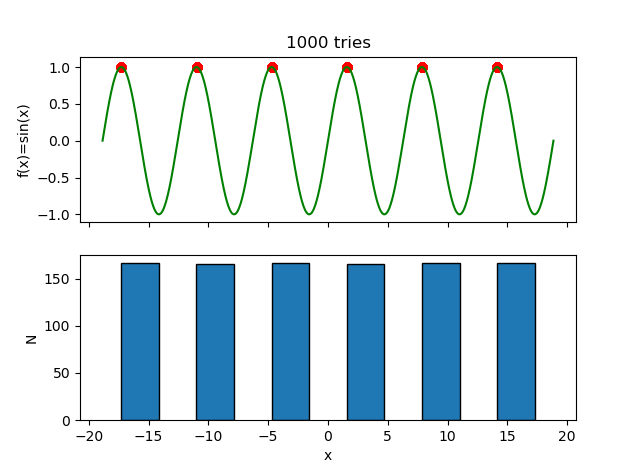
\includegraphics[width=0.9\linewidth]{Q1.png}
\end{figure}

\end{document}